\documentclass[UTF8,zihao=-4]{ctexart}
\usepackage[a4paper,margin=2.5cm]{geometry}
\usepackage{amsmath, amssymb, amsthm}
\usepackage{bm}
\usepackage{hyperref}
\usepackage{graphicx}
\usepackage{caption}
\usepackage{listings}
\usepackage{xcolor}
\usepackage{float}
\usepackage{placeins}
\graphicspath{{figures/}}

% Code style
\lstdefinestyle{code}{
  basicstyle=\ttfamily\small,
  numbers=left,
  numberstyle=\tiny,
  numbersep=8pt,
  keywordstyle=\color{blue},
  commentstyle=\color{teal!70!black},
  stringstyle=\color{orange!70!black},
  showstringspaces=false,
  breaklines=true,
  frame=single,
  framerule=0.3pt,
  rulecolor=\color{black!15}
}
\lstset{style=code}

\title{Transformer 架构:注意力、归一化、位置编码与结构变体}
\author{}
\date{\today}

\begin{document}
\maketitle

\section{注意力机制(Self-Attention, Multi-Head Attention)}
自注意力允许序列中任意位置之间直接建模依赖关系。对输入矩阵 $\mathbf{X} \in \mathbb{R}^{T \times d_{\text{model}}}$,线性映射得到查询、键、值:
\begin{equation}
  \mathbf{Q} = \mathbf{X}\mathbf{W}^Q,\quad \mathbf{K} = \mathbf{X}\mathbf{W}^K,\quad \mathbf{V} = \mathbf{X}\mathbf{W}^V.
\end{equation}
缩放点积注意力的核心公式为
\begin{equation}
  \mathrm{Attention}(\mathbf{Q}, \mathbf{K}, \mathbf{V}) = \mathrm{softmax}\left( \frac{\mathbf{Q}\mathbf{K}^{\top}}{\sqrt{d_k}} \right)\mathbf{V}.
\end{equation}
分母的 $\sqrt{d_k}$ 保持梯度稳定;自回归模型在 softmax 前加上 $-\infty$ 的上三角掩码以屏蔽未来 token。

\subsection{多头注意力}
多头注意力将嵌入空间划分为 $H$ 个子空间,各自执行注意力再拼接:
\begin{align}
  \mathrm{MHA}(\mathbf{X}) &= \mathrm{Concat}(\mathbf{O}_1, \ldots, \mathbf{O}_H)\mathbf{W}^O, \\
  \mathbf{O}_h &= \mathrm{Attention}\left(\mathbf{X}\mathbf{W}_h^Q, \mathbf{X}\mathbf{W}_h^K, \mathbf{X}\mathbf{W}_h^V\right).
\end{align}
多头机制捕捉不同类型的语义关系。常见变体包括:
\begin{itemize}
  \item \textbf{相对位置注意力}(Transformer-XL、T5)在 logits 中加入与距离相关的偏置;
  \item \textbf{稀疏注意力}(Longformer、BigBird、Sparse Transformer)限制感受野以降低复杂度;
  \item \textbf{FlashAttention} 通过块状计算降低显存读写压力,提高精度与速度。
\end{itemize}
图~\ref{fig:self_attention_flow_cn} 展示了多头注意力的整体流程,从线性映射到头间拼接。

\subsection{交叉注意力}
交叉注意力允许查询来自解码器隐藏状态,键/值来自编码器输出:
\begin{equation}
  \mathrm{CrossAttn}(\mathbf{X}, \mathbf{Y}) = \mathrm{Attention}(\mathbf{X}\mathbf{W}^Q, \mathbf{Y}\mathbf{W}^K, \mathbf{Y}\mathbf{W}^V).
\end{equation}
在序列到序列任务中,解码器通过交叉注意力根据编码器信息生成目标序列。

\begin{figure}[H]
  \centering
  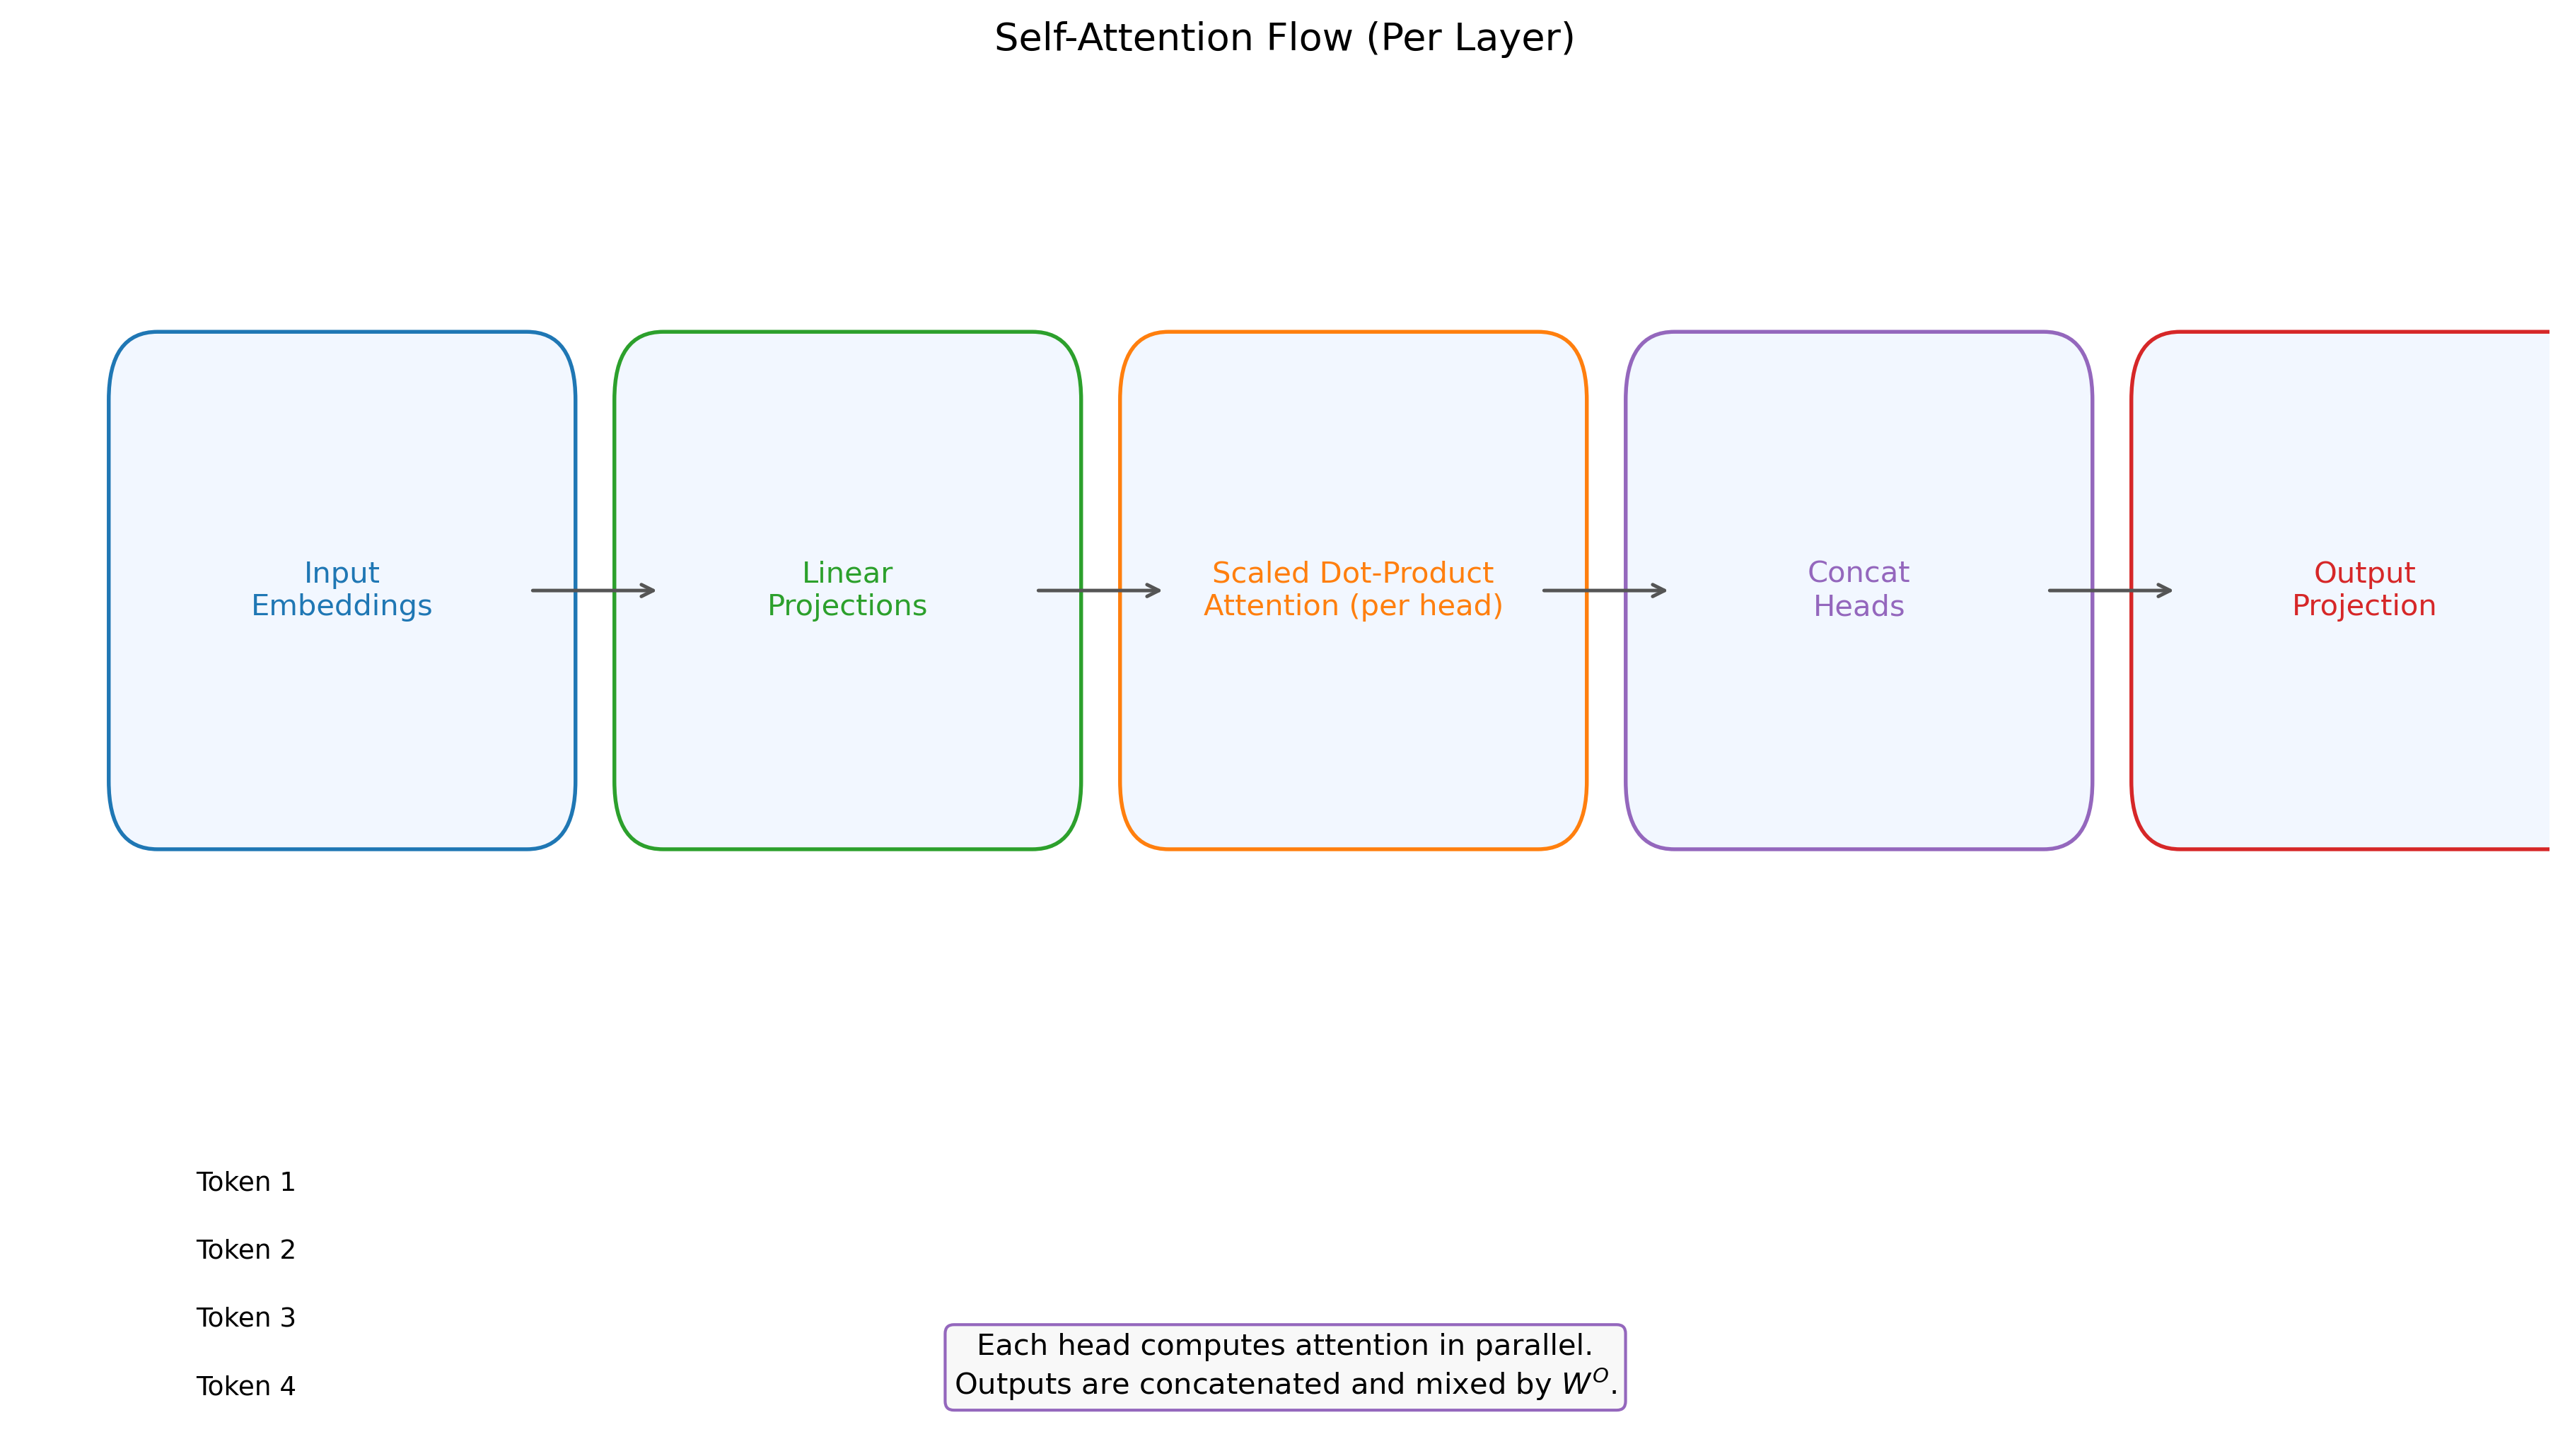
\includegraphics[width=0.85\textwidth]{self_attention_flow.png}
  \caption{多头自注意力流程:查询/键/值投影、逐头注意力、拼接与输出线性组合。}
  \label{fig:self_attention_flow_cn}
\end{figure}
\FloatBarrier

\section{残差连接与层归一化(Residual \& LayerNorm)}
Transformer 依赖残差路径和归一化保持梯度与激活稳定。

\subsection{残差连接}
对任一子层(注意力或前馈网络)应用
\begin{equation}
  \mathbf{y} = \mathbf{x} + \mathrm{Sublayer}(\mathbf{x}).
\end{equation}
残差缓解梯度消失,并允许子层学习对恒等映射的增量调整。预归一化(Pre-LN)结构在子层前执行 LayerNorm,使深层 Transformer 更易收敛。

\subsection{层归一化}
LayerNorm 对每个 token 的特征做归一化:
\begin{equation}
  \hat{\mathbf{h}} = \frac{\mathbf{h} - \mu}{\sqrt{\sigma^2 + \epsilon}},\quad \mathrm{LayerNorm}(\mathbf{h}) = \gamma \odot \hat{\mathbf{h}} + \beta.
\end{equation}
其中 $\mu$、$\sigma^2$ 为特征维度上的均值与方差。LayerNorm 不依赖 batch 大小,适合自回归推理。RMSNorm、ScaleNorm 等变体通过省略偏置或使用均方根归一化来提升稳定性。

\subsection{前馈网络与门控}
位置前馈网络(FFN)通常由两层全连接组成:
\begin{equation}
  \mathrm{FFN}(\mathbf{x}) = \sigma(\mathbf{x}\mathbf{W}_1 + \mathbf{b}_1)\mathbf{W}_2 + \mathbf{b}_2.
\end{equation}
SwiGLU、GEGLU 等门控激活在大模型中表现更好,提升了训练效率和泛化能力。

\section{位置编码(Sinusoidal, RoPE, ALiBi)}
注意力本身与位置无关,需要额外位置编码引入顺序信息。

\subsection{正弦位置编码}
原始 Transformer 使用固定正弦/余弦函数:
\begin{align}
  \mathrm{PE}(t, 2i) &= \sin\left(\frac{t}{10000^{2i/d_{\text{model}}}}\right), \\
  \mathrm{PE}(t, 2i+1) &= \cos\left(\frac{t}{10000^{2i/d_{\text{model}}}}\right).
\end{align}
这种编码可外推到更长序列,并在点积中保留相对位置信息。

\subsection{旋转位置编码(RoPE)}
RoPE 将查询/键向量视为复数,按位置施加旋转:
\begin{equation}
  \mathrm{RoPE}(\mathbf{z}_t) = \mathbf{z}_t \cdot e^{i \theta_t}.
\end{equation}
在实际实现中,对实数向量的偶数/奇数维度成对应用旋转矩阵。RoPE 保留相对位置差值,延长上下文时仍能保持相似的几何关系。

\subsection{ALiBi 偏置}
ALiBi(Attention with Linear Biases)在注意力 logits 中引入随距离线性增长的惩罚:
\begin{equation}
  \mathrm{Score}(i, j) = \frac{\mathbf{q}_i^\top \mathbf{k}_j}{\sqrt{d_k}} - m_h (i - j),
\end{equation}
其中 $m_h$ 为第 $h$ 个头的斜率。ALiBi 无需显式位置编码即可拓展上下文,还可针对不同注意力头设置长短程偏好。

\section{编码器与解码器结构(Encoder-Decoder, Decoder-only)}
\subsection{Encoder-Decoder 架构}
经典 seq2seq Transformer 包含编码器栈和解码器栈。编码器通过多层自注意力与 FFN 将源序列映射为高维表示;解码器在每层执行掩码自注意力、交叉注意力和前馈网络,适用于机器翻译、摘要、语音识别等任务。

\subsection{Decoder-only 架构}
Decoder-only(GPT 系)去掉交叉注意力,仅利用掩码自注意力。其结构简单、便于扩展,适合大规模自回归预训练,并通过提示、few-shot、指令微调等方式支持多种任务。

\subsection{Encoder-only 架构}
Encoder-only(BERT、RoBERTa、DeBERTa)保留双向注意力和残差块,输出上下文嵌入,可直接用于分类、问答、序列标注等理解任务,也常作为特征提取器。

\subsection{混合与扩展}
现代系统常结合不同模块:检索增强模型在 decoder-only 主干添加检索编码器;Prefix tuning、Adapter 等轻量方法为 encoder/decoder 引入任务适配层。图~\ref{fig:transformer_stack_variants_cn} 概述了常见 Transformer 结构形态。

\begin{figure}[H]
  \centering
  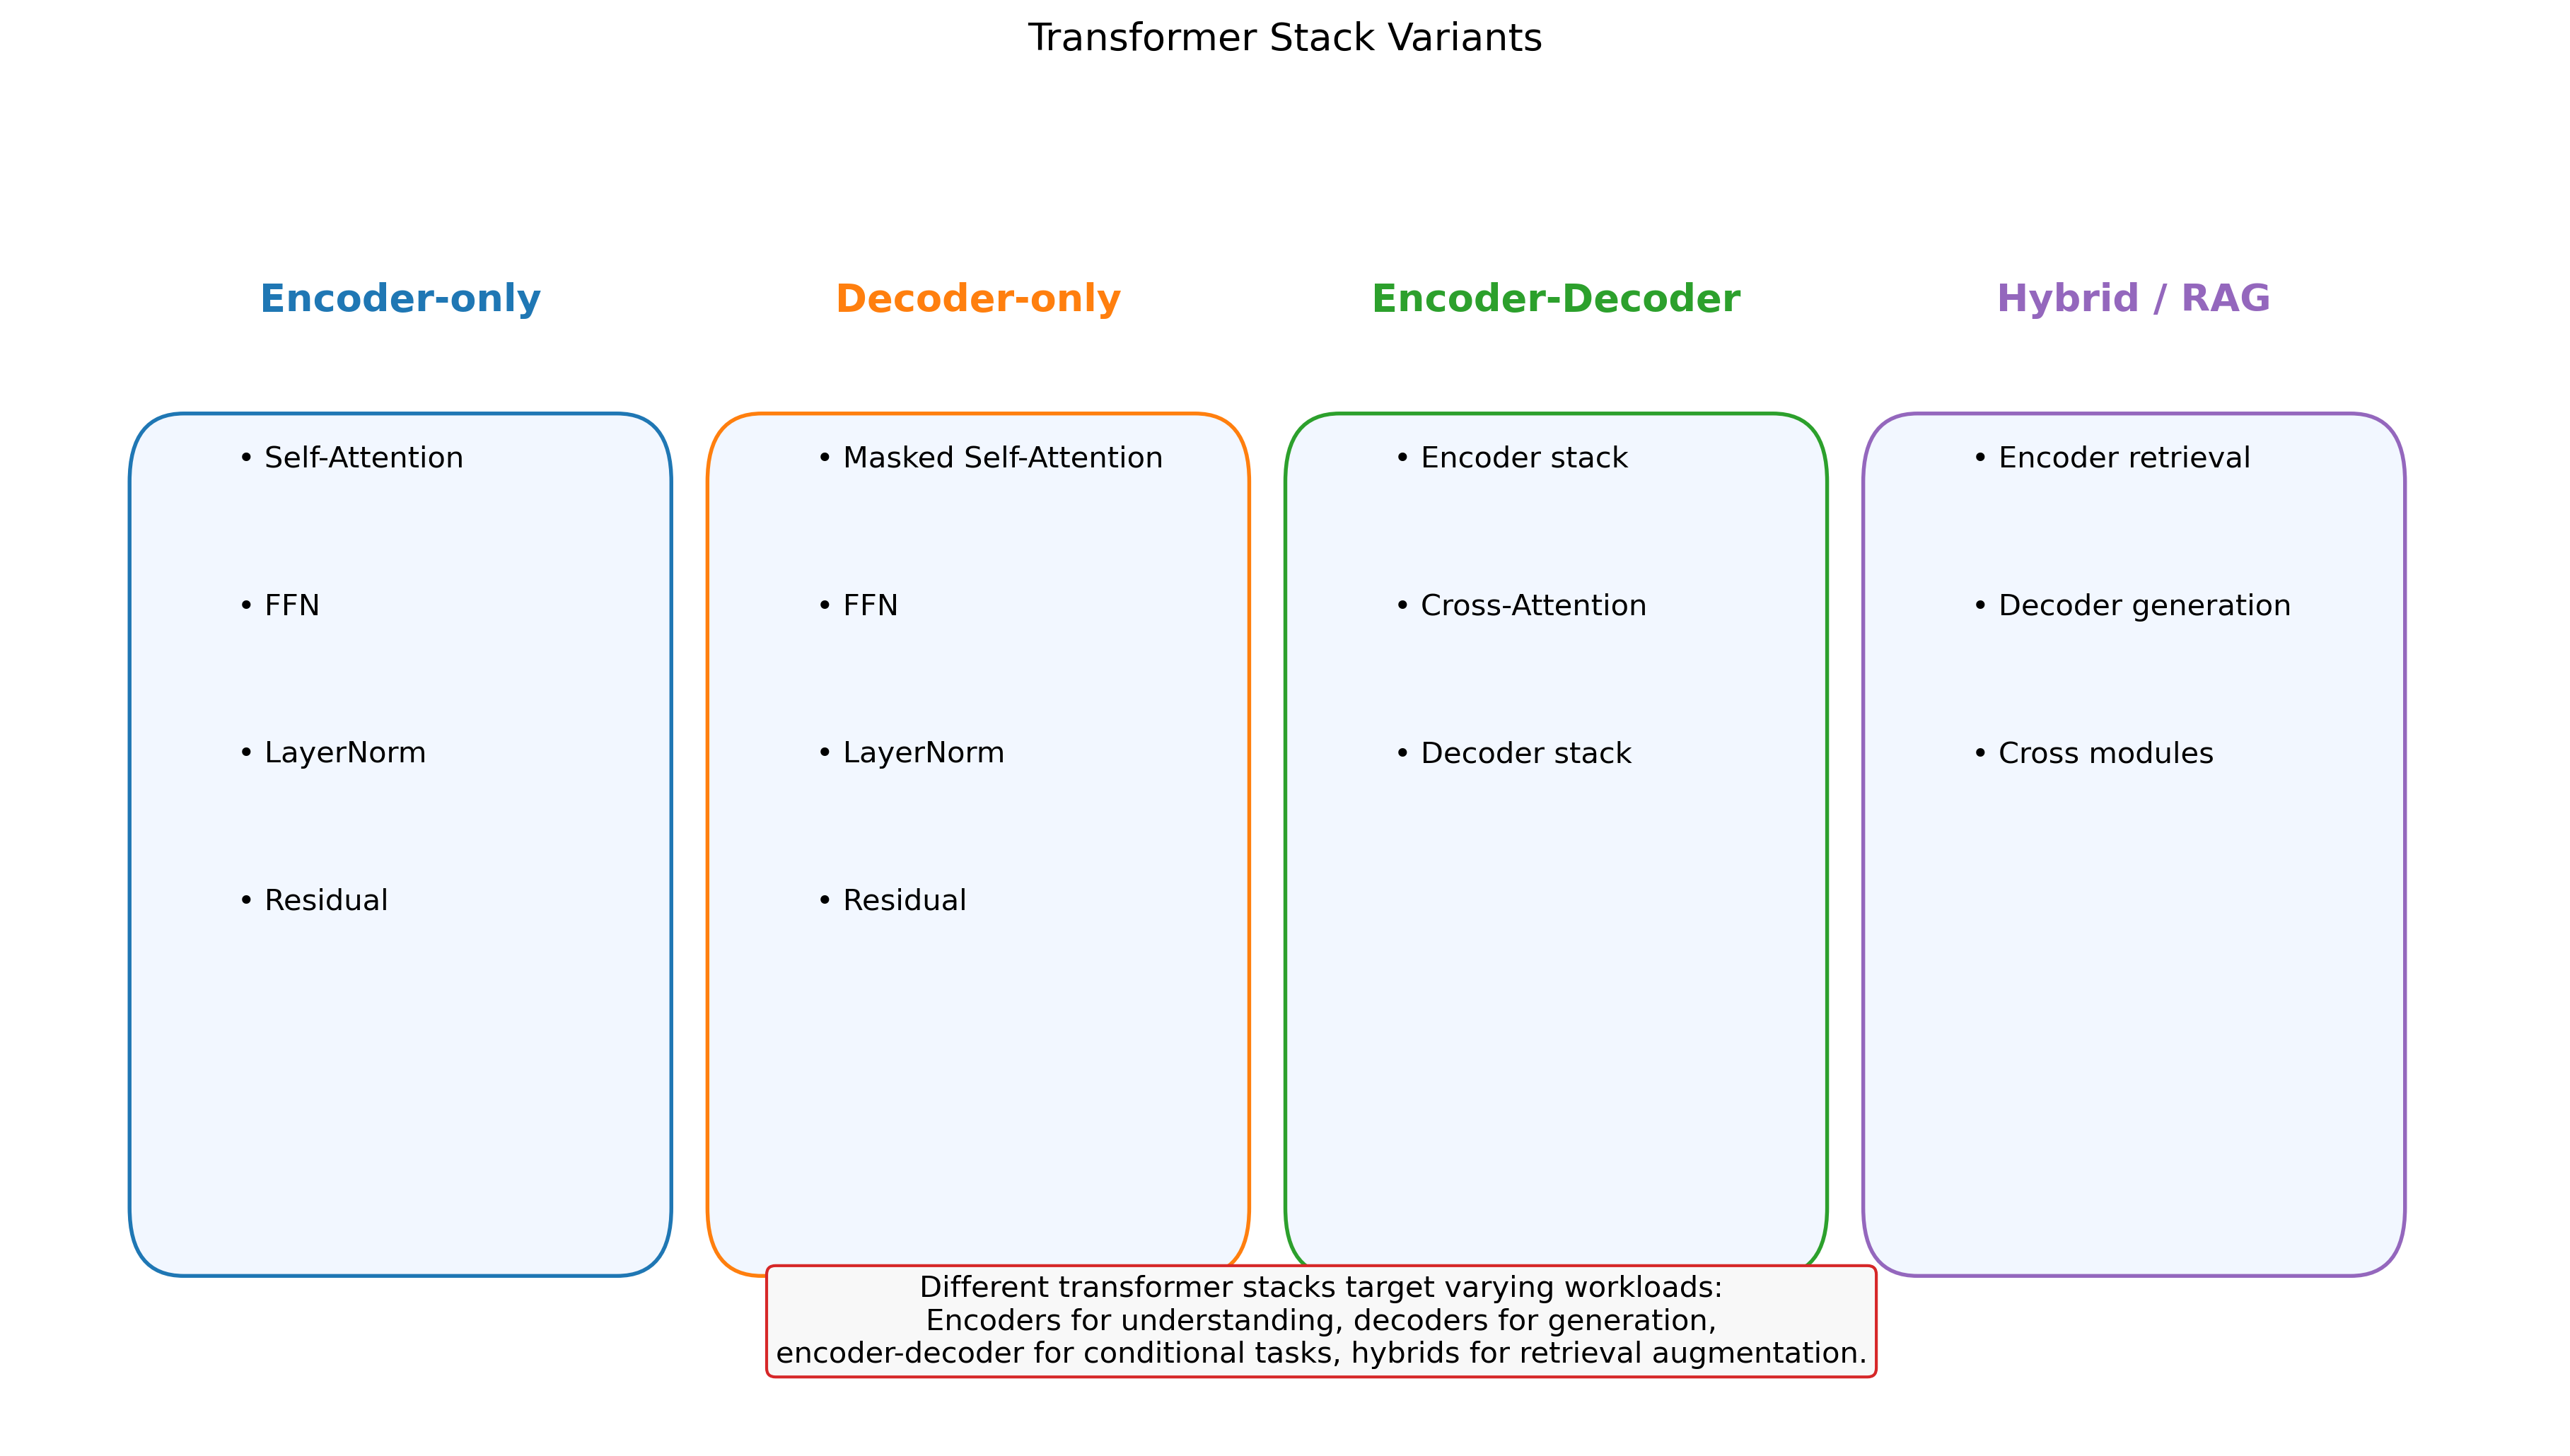
\includegraphics[width=0.9\textwidth]{transformer_stack_variants.png}
  \caption{Transformer 结构形态对比:编码器式、解码器式、编码器-解码器式以及检索增强等混合设计。}
  \label{fig:transformer_stack_variants_cn}
\end{figure}
\FloatBarrier

\section{工程实践提示}
\begin{itemize}
  \item \textbf{规模扩展:} 层数、宽度、头数等超参需与计算预算匹配;预归一化往往优于后归一化以保证深层稳定性。
  \item \textbf{正则与优化:} Dropout、随机深度、权重衰减、梯度噪声等手段可提升泛化;混合精度、FlashAttention 以及流水线/张量并行降低训练和推理成本。
  \item \textbf{部署关注:} INT8/INT4 量化、KV Cache 优化、分层蒸馏等策略可显著降低延迟和显存占用。
\end{itemize}

\section*{延伸阅读}
\begin{itemize}
  \item Vaswani 等:《Attention is All You Need》,NeurIPS 2017。
  \item Shazeer:《Fast Transformer Decoding: One Write-Head is All You Need》,2019。
  \item Xiong 等:《On Layer Normalization in the Transformer Architecture》,ICML 2020。
  \item Press 等:《Train Short, Test Long: Attention with Linear Biases》,ICLR 2022。
  \item Dao 等:《FlashAttention: Fast and Memory-Efficient Exact Attention with IO-Awareness》,NeurIPS 2022。
\end{itemize}

\end{document}
